\documentclass[15pt,a5paper,reqno]{article}
\usepackage{hyperref}
\usepackage[warn]{mathtext}
\usepackage[utf8]{inputenc}
\usepackage[T2A]{fontenc}
\usepackage[russian]{babel}
\usepackage{amssymb, amsmath, multicol}
\usepackage{graphicx}
\usepackage[shortcuts,cyremdash]{extdash}
\usepackage{wrapfig}
\usepackage{floatflt}
\usepackage{lipsum}
\usepackage{verbatim}
\usepackage{concmath}
\usepackage{euler}
\usepackage{xcolor}
\usepackage{etoolbox}
\usepackage{fancyhdr}
\usepackage{subfiles}
\usepackage{enumitem}
\usepackage{amsthm}
\usepackage{indentfirst}
\usepackage{import}

\DeclareMathOperator{\sign}{sign}

\RequirePackage[ left     = 1.5cm,
  right    = 1.5cm,
  top      = 2.0cm,
  bottom   = 1.25cm,
  includefoot,
  footskip = 1.25cm ]{geometry}
\setlength    {\parskip}        { .5em plus .15em minus .08em }
%\setlength    {\parindent}      { .0em }
\renewcommand {\baselinestretch}{ 1.07 }

\fancyhf{}

\renewcommand{\footrulewidth}{ .0em }
\fancyfoot[C]{\texttt{\textemdash~\thepage~\textemdash}}

\makeatletter
\patchcmd\l@section{%
  \nobreak\hfil\nobreak
}{%
  \nobreak
  \leaders\hbox{%
    $\m@th \mkern \@dotsep mu\hbox{.}\mkern \@dotsep mu$%
  }%
  \hfill
  \nobreak
}{}{\errmessage{\noexpand\l@section could not be patched}}
\makeatother
\parindent = 1cm % отступ при красной строке⏎
\pagestyle{fancy}    
\renewcommand\qedsymbol{$\blacksquare$}

\newcommand{\when}[2]{
  \left. #1 \right|_{#2} \hspace
}
\renewcommand{\kappa}{\varkappa}
\RequirePackage{caption2}
\renewcommand\captionlabeldelim{}
\newcommand*{\hm}[1]{#1\nobreak\discretionary{}

\DeclareSymbolFont{T2Aletters}{T2A}{cmr}{m}{it}
{\hbox{$\mathsurround=0pt #1$}}{}}
% Цвета для гиперссылок
\definecolor{linkcolor}{HTML}{000000} % цвет ссылок
\definecolor{urlcolor}{HTML}{799B03} % цвет гиперссылок
 
\hypersetup{pdfstartview=FitH,  linkcolor=linkcolor,urlcolor=urlcolor, colorlinks=true}


%\setcounter{secnum[utf8x]depth}{0}

\begin{document}

% НАЧАЛО ТИТУЛЬНОГО ЛИСТА
\begin{center}
  {\small ФЕДЕРАЛЬНОЕ ГОСУДАРСТВЕННОЕ АВТОНОМНОЕ ОБРАЗОВАТЕЛЬНОЕ\\ УЧРЕЖДЕНИЕ ВЫСШЕГО ОБРАЗОВАНИЯ\\ МОСКОВСКИЙ ФИЗИКО-ТЕХНИЧЕСКИЙ ИНСТИТУТ\\ (НАЦИОНАЛЬНЫЙ ИССЛЕДОВАТЕЛЬСКИЙ УНИВЕРСИТЕТ)\\ ФИЗТЕХ-ШКОЛА РАДИОТЕХНИКИ И КОМПЬЮТЕРНЫХ ТЕХНОЛОГИЙ}\\
  \hfill \break
  \hfill \break
  \hfill \break
  \Huge{Работа 2.2.1. Диффузия}\\
\end{center}

\hfill \break
\hfill \break
\hfill \break
\hfill \break
\hfill \break
\hfill \break

\begin{flushright}
  \normalsize{Работу выполнил:}\\
  \normalsize{\textbf{Долгов Александр Алексеевич, группа Б01-106}}\\
\end{flushright}

\hfill \break
\hfill \break
\hfill \break
\hfill \break
\hfill \break

\begin{center}
  \normalsize{\textbf{Долгопрудный, 2022}}
\end{center}


\thispagestyle{empty} % выключаем отображение номера для этой страницы

% КОНЕЦ ТИТУЛЬНОГО ЛИСТА

\newpage
\thispagestyle{plain}
\tableofcontents
\thispagestyle{plain}
\newpage

\section{Аннотация}

	
	В данной работе исследуется взаимная диффузия газов: гелия и воздуха (более строго, воздух, конечно, является смесью газов). Проводится измерение коэффициента взаимной диффузии этих газов, а также проверяется теоретический результат, что коэффициент взаимной диффузии не зависит от пропорций компонентов бинарной смеси и обратно пропорционален давлению в системе.

\section{Теоретические сведения}

	\textbf{Диффузия} - самопроизвольное взаимное проникновение веществ друг в друга, происходящее вследствие теплового движения молекул.
	Пусть система состоит из двух компонентов: "a"\>и "b". Пусть также диффузия осуществляется только вдоль оси Ox, тогда справедлив закон Фика:
	
	\[j_a = -D\frac{\partial n_a}{\partial x},\>j_b = -D\frac{\partial n_b}{\partial x},\]
	где $j_a$ и $j_b$ - соответственно плотности потока компонентов a и b, то есть число частиц, проходящих через единичную площадку в единицу времени.
	
	Давление P и температура T предполагаются неизменными. Для идеального газа (и гелий и воздух считаем таковыми в условиях эксперимента) справедливо уравнение:
	
	\[P = (n_{He} + n_{air})kT,\]
	где $n_{He}$ и $n_{air}$ - соответственно концентрации гелия и воздуха в сосуде.
	
	Так как $P = const$ и $T = const$, то $n_{He} + n_{air} = const \Rightarrow\ \Delta n_{air} =\\= -\Delta n_{He} \Rightarrow$ достаточно описать диффузию одного из компонентов, например, гелия:
	
	\begin{equation}\label{Helium}
	    j_{He} = -D\frac{\partial n_{He}}{\partial x}
	\end{equation}
	
	В работе предполагается, что $n_{He} \ll n_{air}$. Также верно, что $\mu_{He} \ll\\\ll \mu_{N_2}$ и $\mu_{He} \ll \mu_{O_2}$, то есть атомы гелия значительно легче молекул, из которых в основном состоит воздух. Из этих двух утверждений следует, что процесс взаимной диффузии гелия и воздуха можно приближённо описывать как диффузию примеси лёгких частиц He на практически стационарном фоне воздуха. Для такого приближения верно:
	
	\begin{equation}\label{D_koeff}
	    D = \frac{1}{3}\lambda\overline{v},
	\end{equation}
	где $\overline{v}$ - средняя скорость хаотического движения частиц примеси, $\lambda$ - их длина свободного пробега. Эти величины вычисляются по формулам:
	
	\begin{equation}\label{av_speed}
	    \overline{v} = \sqrt{\frac{8RT}{\pi\mu_{He}}}
	\end{equation}
	\begin{equation}\label{free_run}
	    \lambda = \frac{1}{n_0\sigma},
	\end{equation}
	где $n_0$ - концентрация рассеивающих центров (воздуха в нашем случае), $\sigma$ - сечение столкновения частиц примеси с частицами фона.
	
	В общем случае формула \eqref{D_koeff} также остаётся верна, однако под $\lambda$ нужно понимать величину:
	
	\[\lambda = \frac{1}{(n_{air} + n_{He})\sigma},\]
	а под $\overline{v}$ понимать величину:
	
	\[\overline{v} = \sqrt{\frac{8RT}{\pi\overline{m}}},\]
	где $\overline{m}$ - приведённая масса частиц смеси.
	
	Так как $n_{He} + n_{air} = \frac{P}{kT}$, то $\lambda = \frac{kT}{P\sigma} \Rightarrow D \sim \frac{1}{P}$. Также из приведённых выражения ясно, что величина $D$ не зависеть от пропорций компонентов смеси.
	
\section{Схема эксперимента}
	
	В работе будем использовать сосуды объёмами $V_1$ и $V_2$ ($V_1 \approx V_2 =\\= V$), соединённые трубкой длины L и сечения S. Сосуды заполнены смесью двух газов при одинаковом давлении, но различной концентрации компонентов (рис. 1).
	
	\begin{wrapfigure}{l}{0.25\textwidth}
        \centering
        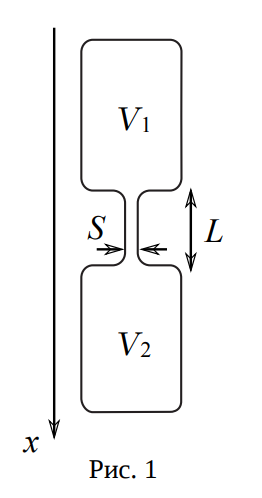
\includegraphics[width=0.25\textwidth]{Рисунок 1.PNG}
    \end{wrapfigure}
	
	В общем случае: $n = n(x, t)$, но если объём соединительной трубки много меньше объёма сосудов ($SL \ll V$), то внутри сосудов можно считать: $n = n(t)$ (концентрация постоянна во всём объёме сосудов) и принять, что концентрация изменяется только благодаря диффузии в трубке.
	
	Сначала предположим, что на концах соединительной трубки концентрации гелия поддерживаются постоянными и равными $n_1$ и $n_2$ (индексы соответствуют индексам объёмов сосудов). Тогда через некоторое время в трубке установится стационарный поток частиц, постоянный во всех сечениях трубки (в противном случае в трубке бы происходило накопление частиц и через некоторое время поток прекратился бы).\\
	Из \eqref{Helium} получаем: 
	\[j = -D\frac{\partial n}{\partial x} = const \Rightarrow \frac{\partial n}{\partial x} = const\]
	
    \noindentОтсюда получаем:
	\begin{equation}\label{concentration}
	    n(x) = \frac{n_2 - n_1}{L}x + n_1
	\end{equation}
	
	\noindentИз \eqref{concentration}: $\frac{\partial n}{\partial x} = \frac{n_2 - n_1}{L}$. Отсюда окончательно получим:
	
	\begin{equation}\label{stream}
	    j = -D\frac{n_2 - n_1}{L}
	\end{equation}
	
	Предположим, что процесс перехода частиц из сосуда 2 в сосуд 1 происходит настолько медленно, что в любой момент времени течение газа можно считать стационарным и описывать формулами \eqref{concentration} и \eqref{stream}, то есть речь идёт о квазистационарном течении.
	
	Также считаем, что концентрация примеси вблизи трубки и в остальных частях сосудов отличаются мало, то есть это отличие много меньше самих концентраций. Тогда в сосудах 1 и 2 соответственно $N_1 = n_1V$ и $N_2 = n_2V$ частиц примеси.
	
	\noindentПо определению плотности потока частиц получаем:
	
	\begin{equation}\label{speed}
	    \frac{dN_1}{dt} = -jS,\>\frac{dN_2}{dt} = jS
	\end{equation}
	
	\noindentЗапишем \eqref{speed} в более удобном виде:
	\[\frac{dn_1}{dt}V = -jS,\>\frac{dn_2}{dt}V = jS \Rightarrow \frac{d}{dt}(n_2 - n_1) = \frac{2jS}{V}\]
	
    \noindentС использованием \eqref{stream} получаем:
    \[\frac{d}{dt}(n_2 - n_1) = -2D\frac{n_2 - n_1}{L}\frac{S}{V}\]
    
    \noindentВведём обозначение: 
    \begin{equation}\label{relax_time}
        \tau = \frac{1}{D}\frac{VL}{2S}
    \end{equation}
    
    \noindentС использованием обозначения получаем:
    \[\frac{d(n_2 - n_1)}{dt} = -\frac{n_2 - n_1}{\tau} \Rightarrow \frac{d(n_2  - n_1)}{n_2 - n_1} = -\frac{dt}{\tau}\]
    
    \noindentРешая последнее уравнение, получаем:
    \begin{equation}
        \Delta n = \Delta n_0 e^{\frac{t}{\tau}},
    \end{equation}
    где $\Delta n \equiv n_2 - n_1$, $\Delta n_0 = \Delta n$ при $t = 0$.
    
	\section{Методика измерений}
    
    Перед проведением измерений необходимо убедиться в соблюдении некоторых условий:\\
    1) Для наблюдения диффузии необходимо отсутствие конвекции $\Rightarrow$ необходимо обеспечить равенство температур и давлений в сосудах до начала эксперимента.\\
    2) Для применения квазистационарного приближения диффузии в трубке необходимо убедиться в том, что величина $\tau \gg \tau_0$ ($\tau_0$ - характерное время диффузии одной частицы вдоль данной трубки). Согласно закону Эйнштейна-Смолуховского: $\tau_0 \sim \frac{L^2}{2D}$.\\
    \[\tau \gg \tau_0 \iff \frac{1}{D}\frac{VL}{S}\gg \frac{L^2}{2D} \iff \frac{V}{S} \gg L \iff SL \ll V\]
    3) Если сосуды расположены вертикально, то влиянием силы тяжести можно пренебречь, так как $mgL \ll kT$.
    
    Для измерения разности концентраций в установке применяются датчики теплопроводности. Теплопроводность $\kappa$ зависит от концентрации: при $\Delta n \ll n_{1, 2}$ можно считать, что $\Delta\kappa = \kappa(n_2) - \kappa(n_1) \approx C\Delta n$, где C - некоторая константа.
    
    Упомянутые датчики в своём устройстве содержат проволоку-нагреватель, приращение сопротивления которой пропорционально теплопроводности газа при заданной мощности тока, текущего по проволоке.
    
    Для измерения сопротивления используется мостовая схема (см. раздел "Экспериментальная установка"), которая балансируется при заполнении сосудов одной и той же смесью. При различии в концентрациях смесей показания вольтметра подсоединённого к диагонали моста: $U \sim \Delta\kappa \sim \Delta n$. Таким образом, в процессе диффузии напряжение изменяется по закону:
    
    \begin{equation}\label{voltage}
        U = U_0 e^{-\frac{t}{\tau}},
    \end{equation}
    где $U_0 = U$ при $t = 0$.
    
    Измеряя $U(t)$, можно найти $\tau$, откуда по формуле \eqref{relax_time} найти коэффициент диффузии D.
    
\section{Экспериментальная установка}
	
	Схема измерительной части установки приведена на рис. 2. Она соединена с системой откачки и напуска воздуха и гелия. Один из вариантов конструкции системы изображён на рис.3.
	
	\begin{figure}[h!]
	    \centering
        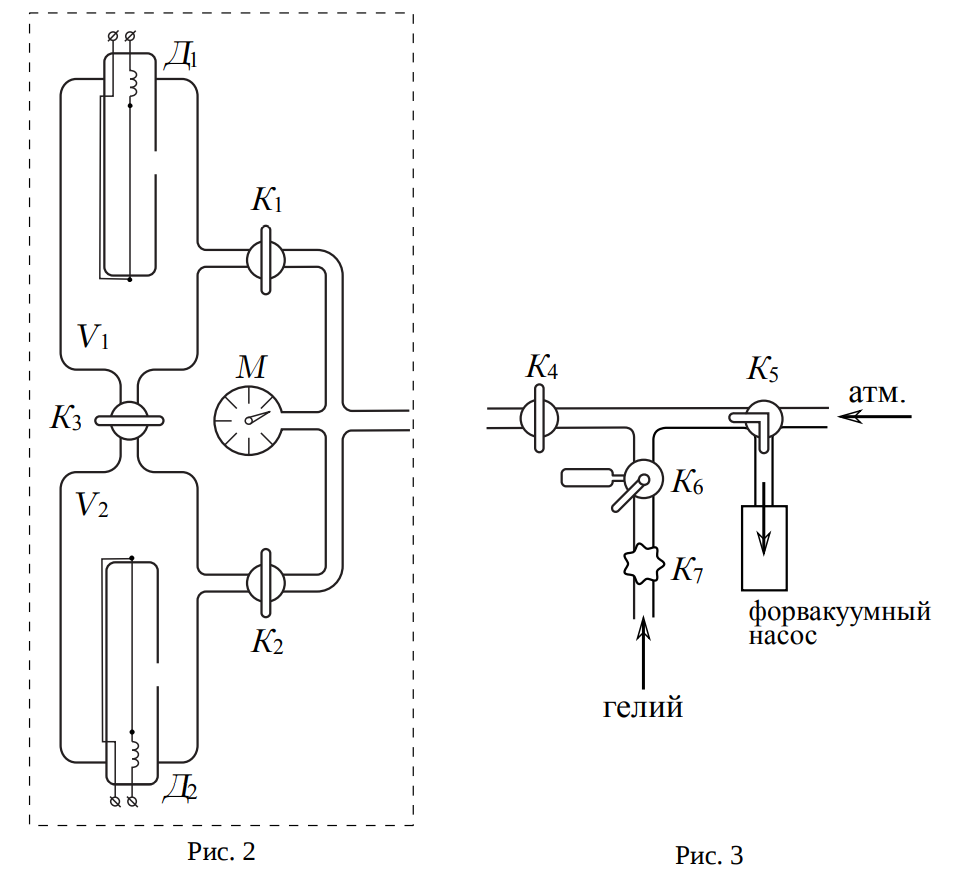
\includegraphics[width = 11cm, height = 10cm]{Рисунки 2 и 3.PNG}
    \end{figure}

	Сосуды $V_1$ и $V_2$ размещены вертикально. Краны $K_1$ и $K_2$ нужны для откачки/подачи гелия в сосуды. Трубка, соединяющая сосуды оснащена краном $K_3$. К соединительным трубкам подключён манометр $M$, измеряющий разность давлений между соединительными трубками и атмосферой. 
	
	\begin{wrapfigure}{r}{0.25\textwidth}
        \centering
        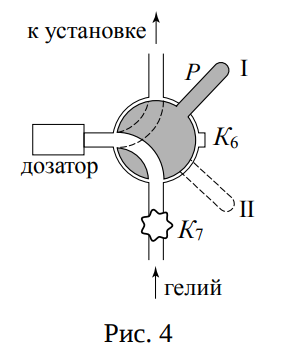
\includegraphics[width=0.25\textwidth]{Дозатор.PNG}
    \end{wrapfigure}
	
	Гелий содержится в баллоне под давлением, превышающем атмосферное. В установке предусмотрен кран $K_7$, отделяющий баллон с гелием от установки. Для подачи малых порций гелия применяется двухходный кран с дозатором (см. рис. 4). Если открыт кран $K_7$ и рычаг $P$ находится в положении $I$, то гелий в небольшом количестве поступает в дозатор. Если $P$ находится в положении $II$, гелий из дозатора поступает в установку.
    
    \begin{wrapfigure}{l}{0.25\textwidth}
        \centering
        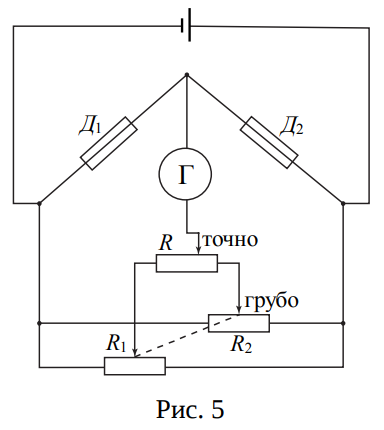
\includegraphics[width=0.25\textwidth]{Мост.PNG}
    \end{wrapfigure}
    
    Датчики теплопроводности $\text{Д}_1$ и $\text{Д}_2$, расположенные в сосудах $V_1$ и $V_2$ соответственно, включены в мостовую схему согласно рис. 5. Резисторы $R$, $R_1$ и $R_2$ служат для балансировки моста. Контакты резисторов $R_1$ и $R_2$ находятся на общей оси и изменяются одновременно поворотом ручки грубой регулировки. Точная балансировка выполняется резистором $R$.\\\\
	
\section{Обработка полученных результатов}

    \noindentПараметры экспериментальной установки:\\
    \[V_1 = V_2 = V = (1200 \pm 30)\text{см}^3\]
    \[\frac{L}{S} = (5,5 \pm 0,5)\text{см}^{-1}\]
    
    Было проведено 4 серии измерений зависимости $U(t)$ при различных значениях давления. Результаты представлены в виде таблиц и графиков (см. раздел "Приложения"). Для каждой серии получено значение $\tau$, полученное аппроксимацией экспериментальных точек графиками вида $y = y_0 + Ae^{-\frac{t}{\tau}}$. Эти значения запишем в табл.1.
    
    \newpage
    \noindentТаблица 1:\\
    \\
    \begin{tabular}{ | l | l | l | }
    \hline
    P, мм рт.ст & $\tau$, c & $\Delta\tau$, c  \\ \hline
    40,4 & 348,8 & $2,4\cdot10^{-5}$ \\ \hline
    80,8 & 522,6 & $6,6\cdot10^{-6}$  \\ \hline
    121,3 & 627,9 & $9,8\cdot10^{-6}$ \\ \hline
    201,4 & 970,1 & $1,2\cdot10^{-5}$ \\
    \hline
    \end{tabular}\\
    
    Обратим внимание на то, что погрешность, отражённая в табл.1 является случайной и её порядок много меньше величины $\tau$. Следовательно, этой погрешностью можно пренебречь и в дальнейших расчётах не учитывать.
    
    \noindentИз \eqref{relax_time} получим, что 
    \[D = \frac{1}{\tau}\frac{L}{S}V\]
    
    Теперь по результатам табл.1 получим значения коэффициента диффузии для каждого значения давления. Также рассчитаем погрешности этих величин. Погрешность $D$ можно посчитать по формуле:
    \[\Delta D = D\sqrt{\left(\frac{\Delta\tau}{\tau}\right)^2 + \left(\frac{\Delta V}{V}\right)^2 + \left(\Delta\left(\frac{L}{S}\right)/\frac{L}{S}\right)^2}\]
    \noindent Так как погрешностью $\Delta\tau$ мы пренебрегли, то последняя формула приобретает вид:
    \[\Delta D = D\sqrt{\left(\frac{\Delta V}{V}\right)^2 + \left(\Delta\left(\frac{L}{S}\right)/\frac{L}{S}\right)^2}\]
    Результаты представим в виде табл.2.\\
    \\
    \noindentТаблица 2:\\
    \\
    \begin{tabular}{ | l | l | l | }
    \hline
    P, мм рт.ст & D, $\text{м}^2/c$& $\Delta D$, $\text{м}^2/c$ \\ \hline
    40,4 & $1,89\cdot10^{-3}$ & $0,2\cdot10^{-3}$ \\ \hline
    80,8 & $1,26\cdot10^{-3}$ & $0,1\cdot10^{-3}$  \\ \hline
    121,3 & $1,1\cdot10^{-3}$ & $0,1\cdot10^{-3}$ \\ \hline
    201,4 & $6,8\cdot10^{-4}$ & $0,6\cdot10^{-4}$ \\
    \hline
    \end{tabular}\\
    \\
    По данным таблицы построим график зависимости $D(\frac{1}{P})$:\\
    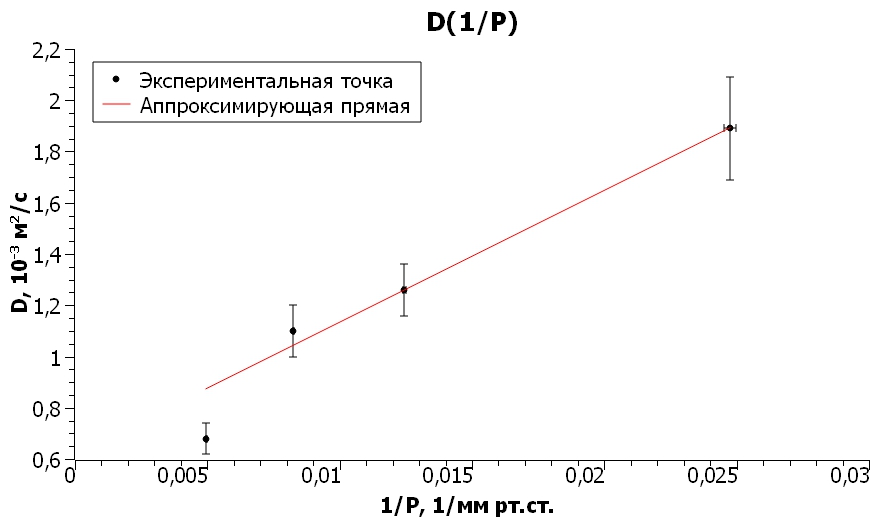
\includegraphics[width = 12cm, height = 7cm]{График.jpg}
    \\
    Погрешность величины $\frac{1}{P}$ можно найти по формуле:
    \[\Delta\left(\frac{1}{P}\right) = \frac{\Delta p}{p^2}\]
    
    Погрешностью измерения давления $\Delta p$ считаем погрешность манометра, которая в для данной экспериментальной установки равна $\Delta p = 50 \text{ Па} \approx 0,38 \text{ мм рт.ст.}$.
    
    Аппроксимируя экспериментальные точки прямой линией, получаем, что угловой коэффициент её наклона равен:
    \[k = (51,5 \pm 5,8)\cdot10^{-3}\frac{\text{м}^2\cdot\text{мм рт.ст.}}{c}\]
    Считая, что зависимость $D(\frac{1}{P})$ имеет вид: $D = \frac{k}{p}$ получим, что при атмосферном давлении ($p = 760\text{ мм рт.ст.}$) коэффициент диффузии равен:
    \[D_{\text{атм}} = (6,8 \pm 0,9)\cdot10^{-5} \frac{\text{м}^2}{c}\]
    Погрешность результата оценивалась по формуле (атмосферное давление считалось точной величиной):
    \[\Delta D_{\text{атм}} = D_{\text{атм}}\frac{\Delta k}{k}\]
    
    Теперь из \eqref{av_speed} и \eqref{free_run} получим формулу для вычисления длины свободного пробега:
    \[\lambda = 3D_{\text{атм}}\sqrt{\frac{\pi\mu_{He}}{8RT}}\]
    Найдём длину свободного пробега молекул гелия в воздухе при температуре $T = 20^{\circ}C = 293K$:
    \[\lambda = (1,6 \pm 0,2)\cdot10^{-7} м\]
    Также справедлива формула:
    \[\sigma = \frac{kT}{P\lambda}\]
    из которой получаем:
    \[\sigma = (2,5\pm 0,3)\cdot10^{-19} \text{м}^2\]
    
\section{Вывод}

    В результате работы вычислено значение коэффициента диффузии гелия в воздухе при атмосферном давлении. Это значение с учётом указанной погрешности соответствует табличным данным: было найдено значение $D_{\text{атм}} = 6,2\cdot10^{-5}\space\frac{\text{м}^2}{c}$. Также найденное значение длины свободного пробега молекулы гелия соответствует табличным значениям с учётом рассчитанной погрешности: было найдено значение $\lambda = 1,75\cdot10^{-7}$. Более того, подтвердилась обратно пропорциональная зависимость коэффициента диффузии от давления газа.
    
\section{Приложения}

    \noindent\textbf{График 1:}\\
    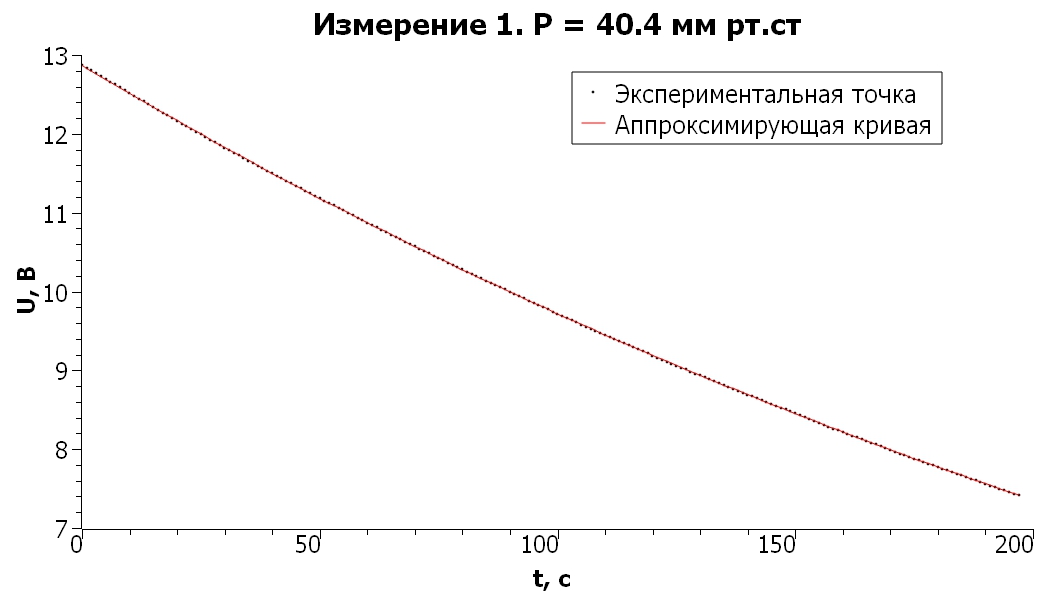
\includegraphics[width = 12cm, height = 7cm]{График 40,4.jpg}\\
    \\
    \noindent\textbf{График 2:}\\
    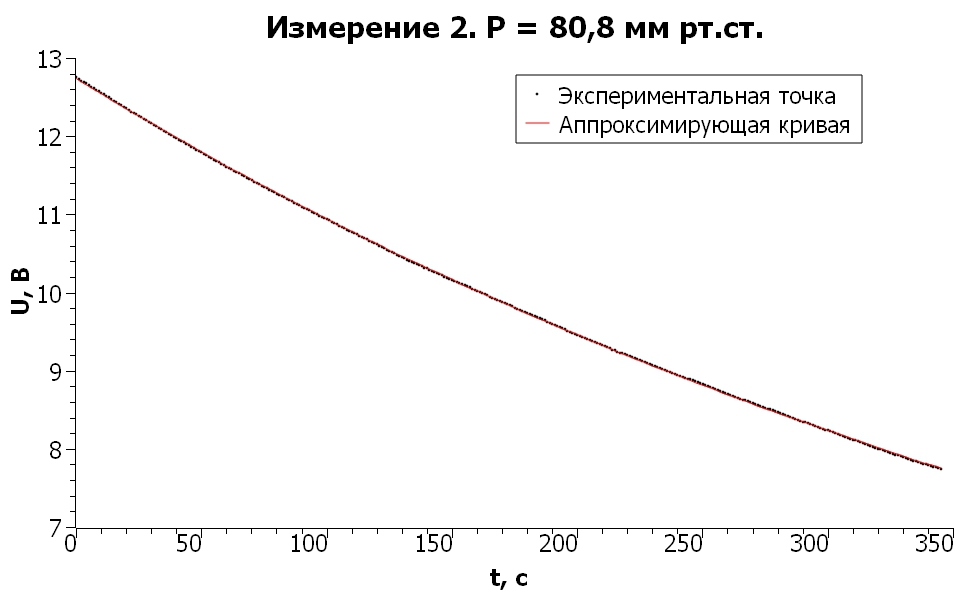
\includegraphics[width = 12cm, height = 7cm]{График 80,8.jpg}\\
    \\
    \noindent\textbf{График 3:}\\
    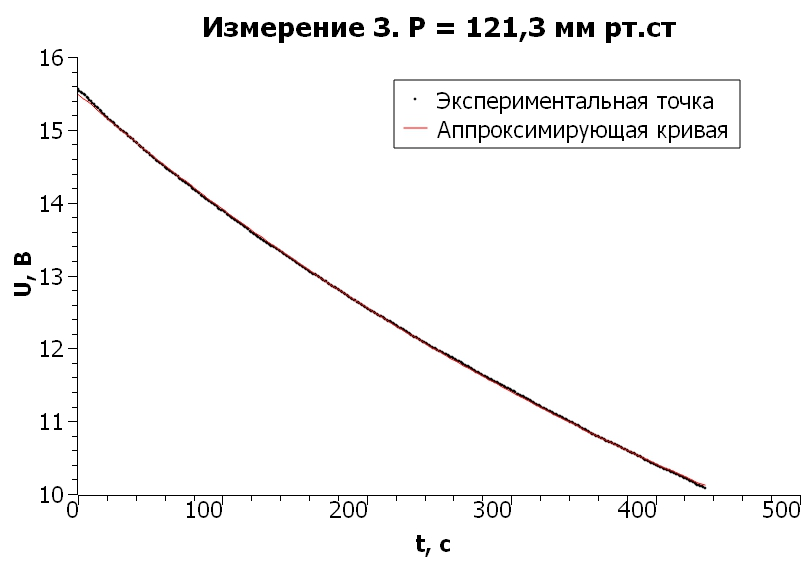
\includegraphics[width = 12cm, height = 7cm]{График 121,3.jpg}\\
    \\
    \noindent\textbf{График 4:}\\
    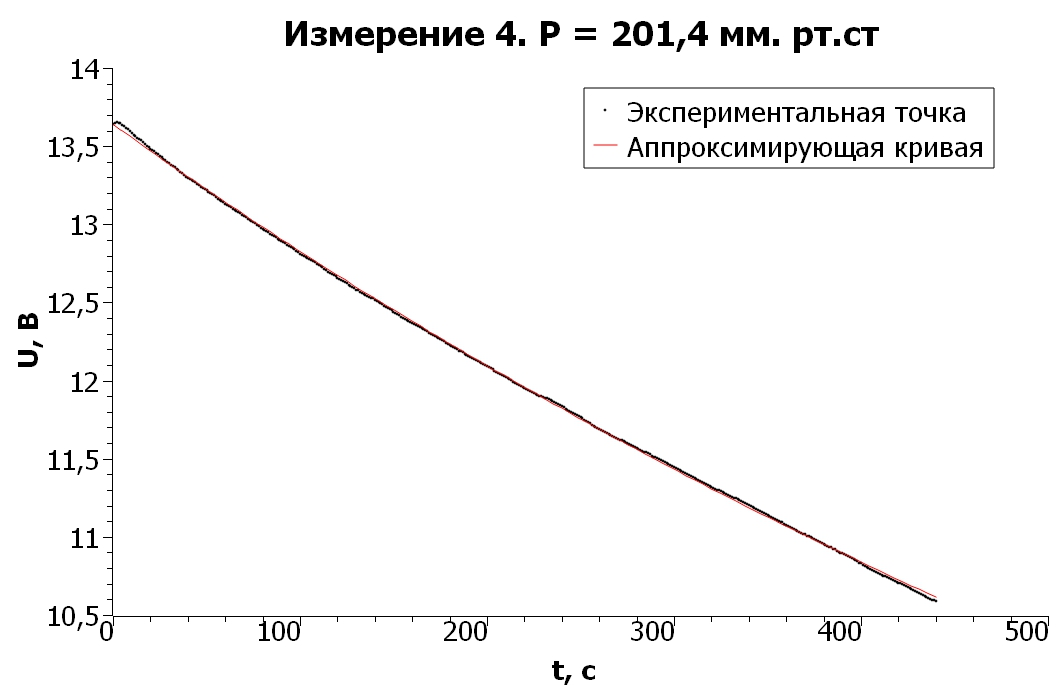
\includegraphics[width = 12cm, height = 7cm]{График 201,4.jpg}\\
    

\end{document}